\documentclass[a4paper]{report}
\usepackage{setspace}

\pagestyle{plain}
\usepackage{amssymb}
\usepackage{graphicx}
\usepackage{color}
\usepackage{amsfonts}
\usepackage{latexsym}
\usepackage{amsmath}
\usepackage[toc,page]{appendix}
\setcounter{tocdepth}{1}
\usepackage{pdfpages}
\usepackage{todonotes}
\usepackage{hyperref}
\hypersetup{
    colorlinks,
    citecolor=black,
    filecolor=black,
    linkcolor=black,
    urlcolor=black
}

\usepackage[authoryear]{natbib}
\usepackage{algorithm}
\usepackage{algpseudocode}

% \usepackage{caption}
\usepackage{subcaption}
\usepackage{float}
\usepackage{lipsum}
\usepackage[a4paper, margin = 3cm, bottom = 2.5cm]{geometry}

\newtheorem{theorem}{THEOREM}
\newtheorem{lemma}[theorem]{LEMMA}
\newtheorem{corollary}[theorem]{COROLLARY}
\newtheorem{proposition}[theorem]{PROPOSITION}
\newtheorem{remark}[theorem]{REMARK}
\newtheorem{definition}[theorem]{DEFINITION}
\newtheorem{example}{Example}

\newcommand{\nats}{\mbox{\( \mathbb N \)}}
\newcommand{\rat}{\mbox{\(\mathbb Q\)}}
\newcommand{\rats}{\mbox{\(\mathbb Q\)}}
\newcommand{\reals}{\mbox{\(\mathbb R\)}}
\newcommand{\ints}{\mbox{\(\mathbb Z\)}}

%%%%%%%%%%%%%%%%%%%%%%%%%%

% ========================================
% Title Page
% ========================================
\title{{\vspace{-14em} 
\includegraphics[scale=0.4]{Logos/ucl_logo.png}}\\
{{\vspace{2em} \Huge Numerical Approximations of the Inverse $\mathbb{Z}$-Transform}}\\
{\large Final Year Project Report}\\
}
\date{Submission date: \today}
\author{Roman Ryan Karim\thanks{
{\bf Disclaimer:}
This report is submitted as part requirement for the MEng degree in Mathematical Computation at UCL. It is substantially the result of my own work except where explicitly indicated in the text. The report may be freely copied and distributed provided the source is explicitly acknowledged.}
\\ \\ Dr Carolyn Phelan
\\ \\ \\ \\ Department of Computer Science
\\ University College London
\\ \\
}


% ========================================
% Report
% ========================================
\begin{document}
 
\onehalfspacing
\maketitle
\begin{abstract}

\end{abstract}

% ========================================
% Contents
% ========================================
\tableofcontents
\setcounter{page}{1}

% ========================================
% Introduction
% ========================================
\chapter{Introduction}
\section{Motivation}

\section{Aims and Objectives}

\section{Overview}

% ========================================
% Background
% ========================================
\chapter{Background}

In Chapter 2, we establish a foundational understanding of the topic in hand. This section is designed to be self-contained, providing essential background for all readers, while references are included for those seeking a deeper exploration.

``By definition, a complex number $z$ is an ordered pair ($x, y$) of real numbers $x$ and $y$, written $z = (x, y)$" \citep{kreyszig2010advanced}. In practice, complex numbers are written in the form $z = x + iy$, where $x$ and $y$ are real numbers and $i$ is the imaginary unit. We may find it easier to represent complex numbers in their polar form, $z = re^{i\theta}$, where $r$ represents the magnitude of $z$ and $\theta$ represents the angle of $z$ with respect to the positive real axis. The set of complex numbers is denoted by $\mathbb{C}$.

% ========================================
% The Z-Transform
% ========================================
\section{The \texorpdfstring{$\mathcal{Z}$}{Lg}-Transform}\label{z_transform}

The $z$-transform is a transformation of a real or complex time function $x(n)$, often used for analyzing discrete-time signals and systems. It is a generalization of the discrete-time Fourier transform (DTFT) that extends the analysis to the complex plane. The Z-transform is formally defined as:

\begin{equation}\label{bilateral_z-transform}
X(z) = \mathcal{Z}_{n \rightarrow z}[x(n)] = \sum^{\infty}_{n = -\infty} x(n)z^{-n}
\end{equation}

\noindent For a convenient description of $z$ in the complex plane, we tend to its polar form $z = re^{i\theta}$.

In the analysis of causal systems - systems for which a time origin is defined and is illogical to consider signal values for negative time - the unilateral $z$-transform is used. Unlike the bilateral $z$-transform in Eq. (\ref{bilateral_z-transform}), we sum from zero to positive infinity yielding

\begin{equation}\label{unilateral_z-transform}
X(z) = \mathcal{Z}_{n \rightarrow z}[x(n)] = \sum^{\infty}_{n = 0} x(n)z^{-n}
\end{equation}

The region within the complex $z$-plane where the $z$-transform converges is known as the Region of Convergence (ROC). The ROC is defined for the set of values of $z$ for which the $z$-transform is absolutely summable

\begin{equation}\label{roc}
\textbf{ROC} = \Biggl\{ z : \sum^{\infty}_{n = 0} |x(n)z^{-n}| < \infty \Biggr\}
\end{equation}

For causal sequences, the ROC is typically the exterior of the outermost pole in the $Z$-plane, denoted as $|z| > a$. If we say that $z_1$ converges, then $z_1$ exists within the ROC. Thus, all $z$ such that $|z| \geq |z_1|$ also converge. This region excludes the poles themselves, as the transform does not converge at those points. For the system to be $stable$, the ROC must include the unit circle, $|z| = 1$, implying that all poles must lie within the unit circle \citep{LovelessGuido2021}.

% ========================================
% Relation to Fourier Transform
% ========================================
\subsection{Relation to the Fourier Transform}\label{rs_fourier_transform}
It is useful to note the relationship between the $z$-transform and the Fourier transform. Taking the Fourier transform of a sampled function $x(t)$ results in:

\begin{flalign}
&& \mathcal{F}\bigg[x(t) \sum^{\infty}_{n = -\infty} \delta(t - n \Delta t)\bigg] &= \int^{\infty}_{-\infty} x(t) \sum_{n = - \infty}^{\infty} \delta (t - n\Delta t)e^{-i \omega t} dt && \\
&& &= \sum_{n = - \infty}^{\infty} \int^{\infty}_{-\infty} x(t) \delta (t - n\Delta t)e^{-i \omega t} dt && \\
&& &= \sum^{\infty}_{n=-\infty} x(n \Delta t)e^{-i \omega nt} &&
\end{flalign}

where we make use of the sifting property of the delta function. If we normalize the sampling interval to 1, we get

\begin{equation}\label{dtft}
\sum^{\infty}_{n = - \infty} x(n)e^{-i n \omega}
\end{equation}

This is the discrete-time Fourier transform (DTFT) of the sequence $x(n)$. The sequence $x(n)$ is sampled at discrete-time intervals $t_n = n \triangle t$, where the sampling interval $\triangle t$ is the time between consecutive samples and the time index $n$ numbers the samples. The DTFT is a periodic function of $\omega$ with period $2\pi$, and its existence relies on the absolute summability of the sequence $x(n)$:

\begin{equation}
\sum^{\infty}_{n = -\infty} |x(n)| < \infty
\end{equation}

The Z-transform generalizes Eq. (\ref{dtft}) to the complex plane, not just the unit circle where $r = 1$ \citep{Oppenheim1989DTSP}.

% ========================================
% Relation to PDFs
% ========================================
\subsection{Relation to Probability Distribution Functions}\label{pdfs}

Random events and signals refer to situations where the outcome is not deterministic, but can be described by probability. Understanding these concepts involves using Probability Distribution Functions; the Probability Mass Function (PMF) for discrete random variables and the Probability Density Function (PDF) for continuous random variables. Given the nature of this project, we'll be focusing our attention on the PMF.

The PMF is defined for a discrete random variable $X$ taking on values $x_i$ with probabilities $p_i$, as $P(X=x_i) = p_i$. The PMF satisfies the following properties:

\begin{equation}
    \sum_{i=0}^n p_i = 1 \hspace{2em}\text{and}\hspace{2em} 0 \leq p_i \leq 1 \hspace{0.5em}\forall i
\end{equation}

We may find it useful to provide a concise representation of the entire distribution such that we expand upon the PMF, $p(x)$, to obtain the Probability Generating Function (PGF), $G_X(q)$, defined as

\begin{equation}
	G_X(q) = E[q^X] = \sum^{\infty}_{x = 0} p(x)q^x,
\end{equation}
where $E[\cdot]$ denotes the expectation operator, and $q$ is a complex number. We deliberately use $q$ to distinguish the PGF from the $z$-transform (Eqn. \ref{z_transform})

% Example using a fair dice
\begin{example}
    Consider a fair six-sided dice. The PMF for the dice roll is given by
    
    \begin{equation}
        p(x) = \begin{cases}
            \frac{1}{6} & \text{if } x = 1, 2, 3, 4, 5, 6 \\
            0 & \text{otherwise}
        \end{cases}
    \end{equation}
    
    where $p(x)$ is the probability of rolling a number $x$. The PGF for the dice roll is then

    \begin{equation}
        G_X(q) = \sum^{\infty}_{x = 0} p(x)q^x = \frac{1}{6} \sum^6_{x = 1} q^x = \frac{q}{6}\cdot \frac{1-q^6}{1-q},
    \end{equation}
    where we use the formula for the sum of a geometric series. The PGF encapsulates the entire distribution of the dice roll into a single function.
\end{example}

The concept of summarizing information is not unique to probability theory. In the analysis of signals, we aim to encapsulate the behaviour of a sequence into a single function. This is akin to the PGF, where the $z$-transform is used to analyze discrete-time signals and systems. Drawing on the principles outlined by \citet{ross2014introduction}, we can bridge the gap between probability theory and signal processing, leveraging the $z$-transform to analyze the behaviour of signals in the complex plane.

% ========================================
% The Inverse Z-Transform
% ========================================
\section{The Inverse \texorpdfstring{$\mathcal{Z}$}{Lg}-Transform}

The inverse $Z$-transform aims to find the $n$-th value of the sequence $x(n)$ given the $Z$-transform $X(z)$. This is commonly defined as a Cauchy integral around a contour $C$ in the complex plane. The contour $C$ is a counter-clockwise closed path that encloses the region of convergence (ROC). The inverse $Z$-transform is formally given by

\begin{equation}\label{inverse_z-transform}
	x(n) = \mathcal{Z}^{-1}_{z \rightarrow n}[X(z)] = \frac{1}{2\pi i} \oint_C X(z)z^{n-1}dz
\end{equation}

In real-world applications, we often require numerical approximation due to computational challenges posed by the Cauchy integral formula. Such approximations enable the effective analysis and processing of complex signals within various technological and financial systems.

% ========================================
% Abate and Whitt 1992
% ========================================
\subsection{Abate and Whitt 1992}
The numerical approximation formula offered by \citet{AbateWhitt1992a, AbateWhitt1992b} is based on a Fourier series catering to the inversion of probability generating functions as elucidated in Section \ref{pdfs}. The format is conducive to queuing theory and other probabilistic models where the $Z$-transform is defined as $q = 1 / z$. The authors approximate the inversion using a trapezoidal rule for numerical integration over a complex contour given by

\begin{equation}\label{aw_inversion_original}
	x(n) \approx \frac{1}{2nr^n} \biggr( X(r) + 2\sum^{n-1}_{k = 1} (-1)^k \mathrm{Re}\bigg( X(re^{\frac{ik\pi}{n}})\bigg) + (-1)^nX(-r) \biggl)
\end{equation}

The parameter $r$ is used to control the error; setting $r = 10^{-\lambda / 2n}$ yields an accuracy bound of $10^{-\lambda}$. The authors leverage the inherent symmetry within the complex plane to enhance computational efficiency by exploiting the complex conjugate symmetry of $X(z)$; each term $X(re^{\frac{ik\pi}{n}})$ in the upper half has a mirror image in the lower half. The computational load is thus halved by \textit{folding} the problem in this manner.

Given the nature of this project, we may find it easier to use the following definition, where we set $z = 1 / q$, to approximate Eq. (\ref{inverse_z-transform}).

\begin{equation}\label{aw_inversion}
	x(n) \approx \frac{1}{2nr^n} \biggr( X(\frac{1}{r}) + 2\sum^{n-1}_{k = 1} (-1)^k \text{Re}\bigg( X\big(\frac{1}{re^{\frac{ik\pi}{n}}}\big)\bigg) + (-1)^nX(-\frac{1}{r}) \biggl)
\end{equation}

The Nyquist-Shannon sampling theorem states that a signal must be sampled at a rate of at least twice the highest frequency present in the signal to avoid aliasing \citep{shannon1949communication,nyquist1928certain}. The number of points, $n$, used in Eqn. (\ref{aw_inversion}) must be sufficient to capture the significant frequency components. If $n$ is too small, the approximation may lead to inaccuracies - akin to aliasing in signal processing.

% ========================================
% Cavers 1978
% ========================================
\subsection{Cavers 1978}
Extending upon our analysis in Section \ref{rs_fourier_transform}, \citet{Cavers1978FFT} proposes to sample the $z$-transform of a function on a circular contour at equally spaced points and then apply the inverse FFT to these sampled points to approximate the original time-domain signal. We can formulate this as:

\begin{equation}\label{cavers}
	f(n) = r^n \text{IFFT}[f(re^{2\pi i / N})],
\end{equation}

where $r$ is the radius of the circular contour, $n$ is the time index, and $N$ is the number of points used in the DFT. The factor $r^n$ scales the result appropriately based on the radius of the contour.

\todo[inline]{Mention the $\frac{1}{N}\text{FFT}$ version as FFT is a fast way to compute DFT - Parseval's theorem? Should I mention in Experimentation when I use MatLab/Python?}

\subsection{Series acceleration techniques}

\section{Option Pricing}
The concept involves determining the value of options, which are financial contracts that give the holder the right, \textit{but not the obligation}, to buy or sell an asset at a set price within a specified time-frame. The value of an option is derived from the underlying asset, which can be a stock, bond, or commodity. 

A pivotal point in option pricing was the introduction of \citet{black1973pricing}'s model in estimating the price of European-style options, which can only be exercised at the expiration date. The Black-Scholes model is based on the assumption that the price of the underlying asset follows a geometric Brownian motion with constant volatility, risk-free interest rate and no transaction costs. However, many options traded in real markets are American-style, allowing the holder to exercise the option at any time before the expiration date. This complicates the pricing process as it involves solving an \textit{optimum stopping problem}. \citet{merton1973theory} extends the Black-Scholes model to American options by expressing the price as the solution to a free boundary problem. While Merton's work provided a theoretical foundation, solving the free boundary problem analytically is challenging. Instead, numerical methods such as binomial trees \citep{cox1979option} and simulation-based methods \citep{longstaff2001simulation} have been developed to price American options.

\subsection{Discrete Monitoring}
In most cases, the payoff of an option depends on the price of the underlying asset at discrete points in time rather than continuously. This is known as discrete monitoring. Two widely traded types of discretely monitored options are lookback and barrier options \citep{dadachanji2015fx}. These options are classified as \textit{exotic options} where the payoff is based on the path of the underlying asset price rather than just the price at expiration.

\begin{enumerate}
    \item \textbf{Barrier Options}
    
    The payoff depends on whether the price of the underlying asset reaches a certain level (the barrier) during the life of the option. A \textit{knock-in} barrier option only come into existence if the barrier has been touched, while a \textit{knock-out} barrier option ceases to exist instead. For example, a \textit{down-and-out} barrier option is a type of knock-out option that becomes worthless if the price of the underlying asset falls below the barrier level. On the other hand, a \textit{down-and-in} barrier option is a type of knock-in option that only becomes active if the asset price falls below the barrier level.

    \item \textbf{Lookback Options}
    
    The payoff depends on the maximum and minimum asset price over the life of the option. A \textit{lookback call option} gives the holder the right to buy the asset at the lowest price during the option period, while a \textit{lookback put option} allows the holder to sell the asset at the highest price during the option period.
\end{enumerate}

% \subsubsection{Barrier Options}
% An exotic option where the payoff depends on whether the price of the underlying asset reaches a certain level (the barrier) during the life of the option. A \textit{knock-in} barrier option only come into existence if the asset price is breached, while a \textit{knock-out} barrier option ceases to exist if the barrier is hit.

% For example, a \textit{down-and-out} barrier option is a type of knock-out option that becomes worthless if the price of the underlying asset falls below the barrier level. On the other hand, a \textit{down-and-in} barrier option is a type of knock-in option that only becomes active if the asset price falls below the barrier level.

% \subsubsection{Lookback Options}
% An option where the payoff depends on the maximum and minimum asset price over the life of the option. A \textit{lookback call option} gives the holder the right to buy the asset at the lowest price during the option period, while a \textit{lookback put option} allows the holder to sell the asset at the highest price during the option period.

\subsection{Use of Fourier Transforms}
However, the pricing of these options can be computationally expensive due to the high-dimensional integrals involved in the pricing formulas. \citet{carr1999option} was the first to propose using Fourier transforms to price European options. It involved transforming the pricing problem from the time domain to the frequency domain, where the pricing formula simplifies to a one-dimensional integral.

\begin{itemize}
    \item talk about the advancements of Fourier transforms in option pricing
    \item mention the linear dependence of the investigated ways
    \item lead on to Fusai et al. (2006)
    \item look into Plancherel's theorem
    \item talk about Phelan's extension
    \item end off with why we're looking into the inverse Z-transform
\end{itemize}

\section{Optimization Techniques}
In the context of computational mathematics, optimizations techniques are used to identify the optimal or a sufficiently effective solution to a problem within a given set of constraints. The goal is to minimize or maximize a specific objective function by systematically choosing the values of the variables. The objective function is often referred to as the \textit{cost function} or \textit{loss function} and the variables are referred to as \textit{parameters}. The optimization problem can be formulated as

\begin{equation}\label{optimization_problem}
	\text{minimize } f(x) \text{ subject to } x \in \Omega
\end{equation}

where $f(x)$ is the objective function and $\Omega$ is the feasible region defined by the constraints of the problem.

Gradient descent is one of the most popular algorithms for parameter optimization with success in Deep Learning and Neural Networks employing variants of the algorithm \citep{lu2017improved, zhang2019gradient, zeebaree2019trainable}. The adaptability to diverse problem domains \citep{YingjieYugiHaibin2023SGD} parallels our use case, where gradient descent is applied outside traditional deep learning to optimize parameters of a mathematical function \citep{GradientBasedOpt2022}.

% ========================================
% Gradient Descent
% ========================================
\subsection{Gradient Descent}
Gradient descent iteratively converges to a local minimum of a function by moving in the direction of the steepest descent, as defined by the negative gradient. This method is expressed mathematically as

\begin{equation}\label{GD}
    x_{k+1} = x_k - \alpha_k \nabla f(x_k)
\end{equation}

where $x_k$ is the parameter vector at iteration $k$, $\alpha_k$ is the learning rate, and $\nabla f(k)$ represents the gradient of the function at $x_k$. The selection of $\alpha_k$ determines the size of the step taken towards the minimum; too large can overshoot the minimum, too small can result in a long convergence time. The process repeats until a predetermined termination criterion is met, typically when the change in the value of $f(k)$ falls below a threshold. This iterative process is showcased in the pseudocode below:

\begin{algorithm}
\caption{Gradient Descent}
\begin{algorithmic}[1]
\State Initialize \( x_0 \), set \( k = 0 \)
\While{termination conditions not met}
    \State Compute gradient \( \nabla f(x_k) \)
    \State Choose a suitable step size \( \alpha_k \)
    \State Update \( x_{k+1} = x_k - \alpha_k \nabla f(x_k) \)
    \State \( k = k + 1 \)
\EndWhile
\end{algorithmic}
\end{algorithm}

% ========================================
% Stochastic Gradient Descent
% ========================================
\subsubsection{Stochastic Gradient Descent}

However, classic Gradient Descent faces limitations, including susceptibility to local minima and potential for overshooting or long convergence times. Stochastic Gradient Descent (SGD) addresses these issues by introducing variability in the optimization process. It modifies Eq. (\ref{GD}) to use a randomly selected subset of data to compute the gradient, to allow for dynamic adjustment of the learning rate and leveraging noise to escape local minima. We define the update rule to 

\begin{equation}\label{SGD}
x_{k+1} = x_k - \alpha_k \nabla f_{i_k}(x_k)	
\end{equation}
where $\nabla f_{i_k}(x_k)$ is the gradient of the cost function with respect to a random subset $i_k$. We thus avoid the pitfalls associated with a static learning rate and promote a quicker convergence time.

\todo[inline]{Time isn't a big factor - but if it is, SGD with momentum can be used so talk about it here (include diagram)}

% ========================================
% Experiment
% ========================================
\chapter{Experiment}

\section{Levendorskii's Sinh Deformation}

\subsection{Deforming the Contour}

\subsection{Parameter Grid Search}

\section{Benchmarking the Approximation Methods}

% ========================================
% Results
% ========================================
\chapter{Results}

% ========================================
% Conclusion
% ========================================
\chapter{Conclusion}
\section{Summary}

\section{Future Work}

\section{Acknowledgements}


% ========================================
% References 
% ========================================
\addcontentsline{toc}{chapter}{References}
\bibliography{references}
\bibliographystyle{apalike}

% ========================================
% Appendix
% ========================================
\begin{appendices}

\chapter{Initial Project Plan}

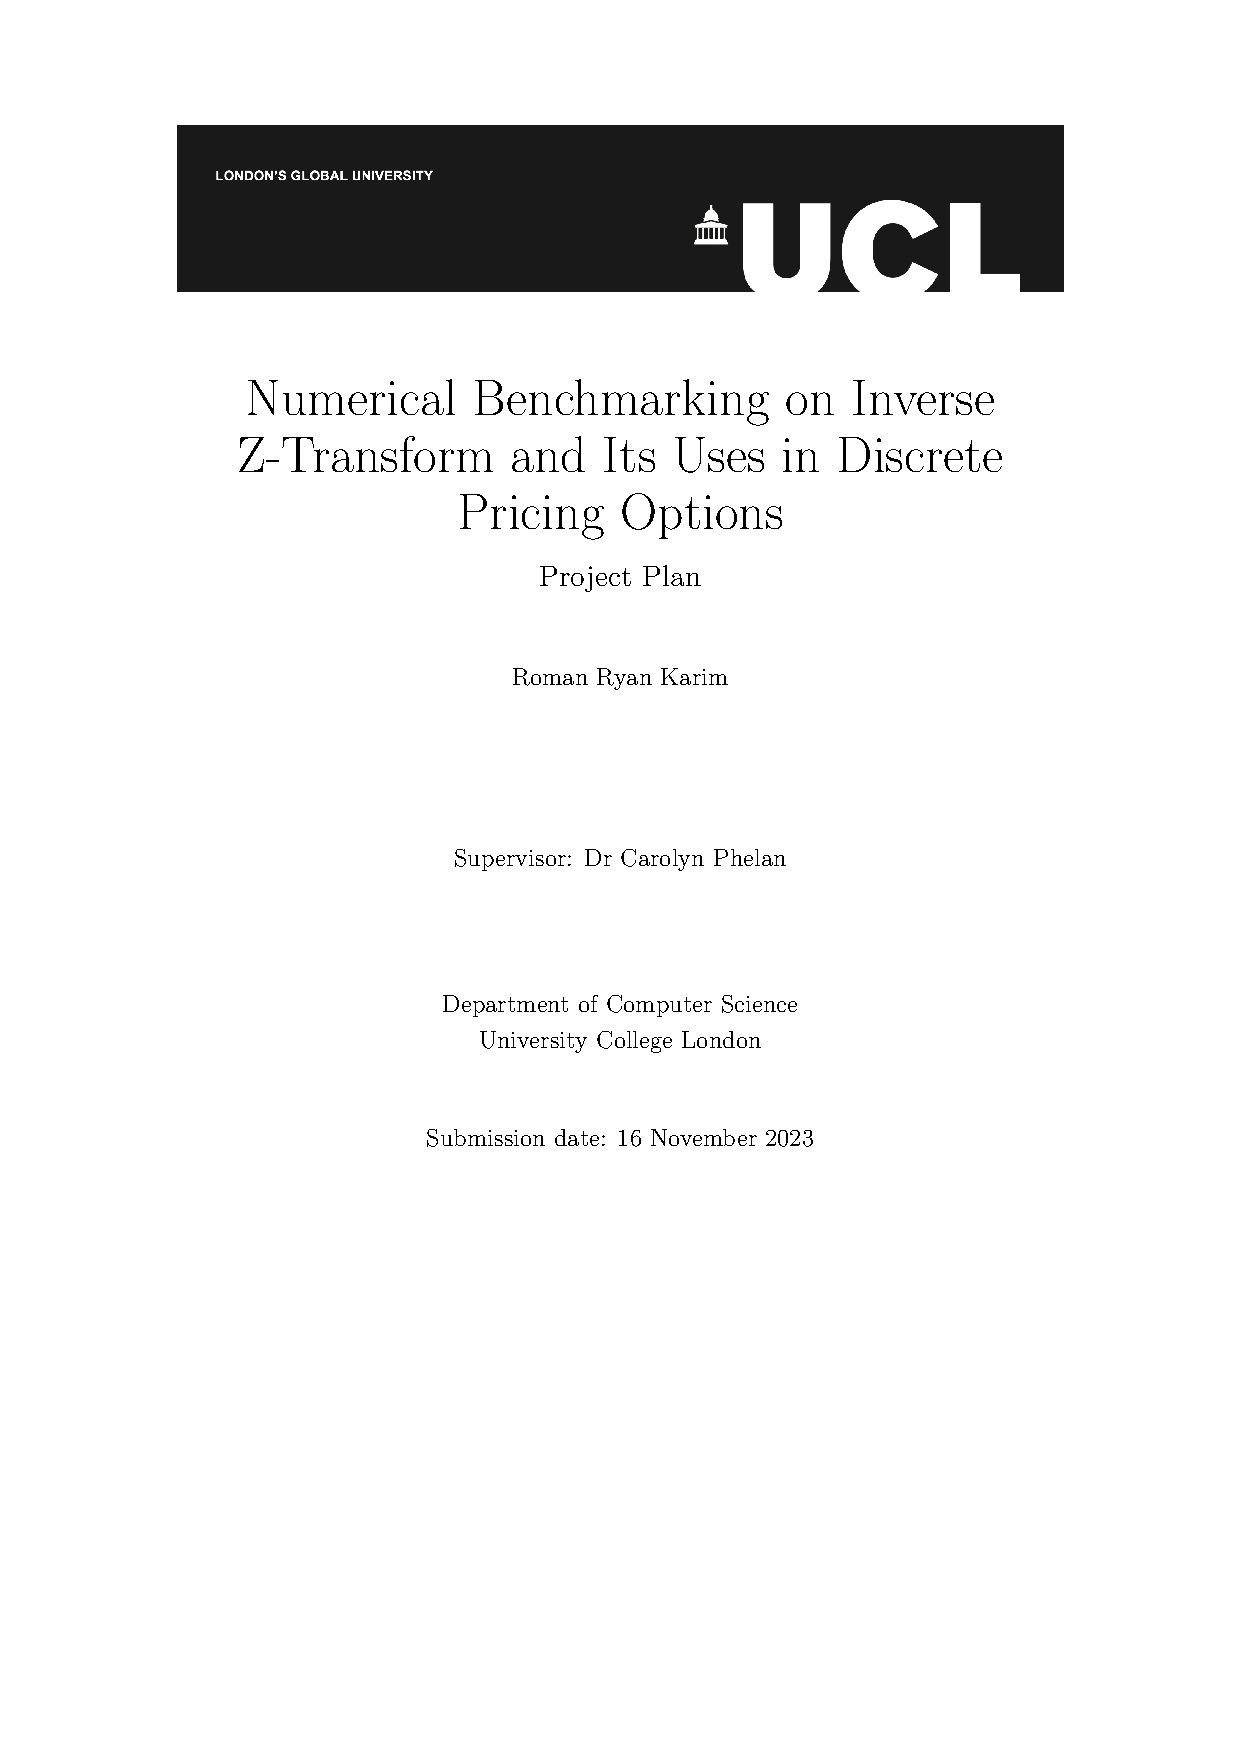
\includepdf[pages=-]{initial_project_plan.pdf}
    
\end{appendices}

\end{document}